%% ---------------------------------------------------------------------------
%%  Supplementary Material for the Neurocomputing submission.
%%
%%  This file is a standalone document. It collects the supporting tables and
%%  figures that are cited from the main manuscript but not printed there, so
%%  the main text stays focused while every number remains available to the
%%  reviewer.
%%
%%  Build:  latexmk -pdf supplementary.tex
%% ---------------------------------------------------------------------------
\documentclass[1p,10pt]{elsarticle}

\usepackage[utf8]{inputenc}
\usepackage[T1]{fontenc}
\usepackage{amsmath,amssymb}
\usepackage{newtxtext}
\usepackage{newtxmath}
\usepackage{graphicx}
\usepackage{float}
\usepackage{booktabs}
\usepackage{multirow}
\usepackage{adjustbox}
\usepackage{url}
\usepackage{microtype}
\usepackage[hidelinks]{hyperref}
\usepackage{xurl}

\setlength{\emergencystretch}{2em}
% Single-column layout: allow floats to share pages instead of one per page.
\renewcommand{\topfraction}{0.92}
\renewcommand{\bottomfraction}{0.85}
\renewcommand{\textfraction}{0.08}
\renewcommand{\floatpagefraction}{0.72}
\setcounter{topnumber}{3}
\setcounter{bottomnumber}{2}
\setcounter{totalnumber}{4}

\newcommand{\modelname}{\textsc{SCORE-Net}}
\newcommand{\R}{\mathbb{R}}

% Supplementary floats and sections are numbered S1, S2, ...
\renewcommand{\thesection}{S\arabic{section}}
\renewcommand{\thetable}{S\arabic{table}}
\renewcommand{\thefigure}{S\arabic{figure}}

\journal{Neurocomputing}

% The supplement is single-column, so a two-column float environment is
% unnecessary. Map table* onto table to keep the tables flowing with the text
% instead of stacking them one per page.
\makeatletter
\renewenvironment{table*}[1][t]{\begin{table}[#1]}{\end{table}}
\makeatother

\begin{document}

\begin{frontmatter}

\title{Supplementary Material for\\ \modelname: Inherently Interpretable
Tabular Classification via Localized Convex Slabs}

\author[a]{Ahmet Alkan\corref{cor1}}
\ead{ahmetalkan@sakarya.edu.tr}
\author[a]{Gozde Yolcu Oztel}
\ead{gyolcu@sakarya.edu.tr}
\cortext[cor1]{Corresponding author.}
\address[a]{Department of Software Engineering, Faculty of Computer and
Information Sciences, Sakarya University, Esentepe Campus, 54187 Serdivan,
Sakarya, Turkey}

\begin{abstract}
This supplement supports the main manuscript with four tables (dataset summary,
protected-attribute ablation, offline training cost, full baseline-latency
comparison) and six figures that the main text cites but does not print. All
values are produced by the released code from the same seeds and splits as the
main results, and no number differs from the reporting in the main manuscript.
\end{abstract}

\end{frontmatter}

% Keep floats off the title page; in single-column mode the first table can
% otherwise be placed above the front matter.
\suppressfloats[t]


\section{Datasets and Splits}
\label{sec:supp_datasets}

Table~\ref{tab:dataset_summary} lists the benchmark datasets and the training,
validation and test partitions used throughout. The table is provided here
because the same information is already given in the dataset list of the main
text, which also describes the splitting protocol.

\begin{table*}[t]
\centering
\footnotesize
\caption{Summary of benchmark datasets. Train/validation/test counts follow the stratified protocol registered for each dataset (COMPAS: 72/8/20; German Credit: 80/10/10; UCI Adult: 72/8/20; Synthetic: 72/8/20).}
\label{tab:dataset_summary}
\renewcommand{\arraystretch}{1.2}
\setlength{\tabcolsep}{6pt}
\adjustbox{max width=\linewidth}{%
\begin{tabular}{l ccccc l}
\toprule
\textbf{Dataset} & \textbf{Samples ($M$)} & \textbf{Features ($N$)} & \textbf{Classes ($C$)} & \textbf{Train / Val / Test} & \textbf{Test Share} & \textbf{Domain} \\
\midrule
COMPAS & 7,214 & 13 & 2 & 5,193 / 578 / 1,443 & 20\% & Criminal Justice \\
German Credit & 1,000 & 48 & 2 & 800 / 100 / 100 & 10\% & Credit Underwriting \\
UCI Adult & 45,222 & 97 & 2 & 32,559 / 3,618 / 9,045 & 20\% & Socio-Economic \\
Synthetic & 20,000 & 30 & 20 & 14,400 / 1,600 / 4,000 & 20\% & Multiclass Benchmark \\
\bottomrule
\end{tabular}
}%
\end{table*}


\section{Protected-Attribute Ablation}
\label{sec:supp_protected}

Table~\ref{tab:protected_ablation} repeats the cross-validated comparison with
the one-hot \texttt{sex\_*} and \texttt{race\_*} columns removed from COMPAS.
Only the feature set changes; the split ratios and pruned-model hyperparameters
are identical to the main benchmark. The Global Best variant is essentially
unchanged, and the Compact variant loses about one point, so the protected
attributes carry almost no predictive signal on this dataset.

\begin{table}[t]
\centering
\footnotesize
\caption{Removing the legally protected attributes from COMPAS. Split ratios and hyperparameters are unchanged; only \texttt{sex\_*} and \texttt{race\_*} are dropped, leaving 7 instead of 13 inputs. Values are $5\times5$ cross-validated test accuracy and $\Delta$ is the paired per-fold difference to the strongest baseline.}
\label{tab:protected_ablation}
\setlength{\tabcolsep}{1.5pt}
\adjustbox{max width=\linewidth}{%
\begin{tabular}{l l r c l c c}
\toprule
\textbf{Feature set} & \textbf{Variant} & \textbf{$N$} & \textbf{CV Acc (\%)} & \textbf{Best baseline} & \textbf{$\Delta$ (pp)} & \textbf{Folds} \\
\midrule
All features & Global Best & 13 & 67.56$\pm$1.49 & CatBoost & -0.38 & 9/25 \\
All features & Compact & 13 & 66.81$\pm$1.66 & CatBoost & -1.13 & 5/25 \\
No sex/race & Global Best & 7 & 67.67$\pm$1.35 & EBM (InterpretML) & -0.43 & 3/25 \\
No sex/race & Compact & 7 & 65.62$\pm$2.42 & EBM (InterpretML) & -2.47 & 2/25 \\
\bottomrule
\end{tabular}
}
\end{table}


\section{Offline Training Cost}
\label{sec:supp_train_cost}

Table~\ref{tab:train_cost} reports the wall-clock cost of a complete pruning
trajectory (base fit plus 14--20 pruning stages) and compares it with the median
and minimum fit time of the 13 baselines on the same folds. The SCORE-Net times
were recorded by the cross-validation runner on CUDA when a GPU was available,
and the baseline times on the CPU, so the table supports an order-of-magnitude
statement rather than a controlled hardware comparison.

\begin{table}[!b]
\centering
\footnotesize
\caption{Offline training cost. \modelname{} is the mean $\pm$ standard deviation of the full pruning trajectory (base fit plus 14--20 stages); per stage divides this by the number of stages. Baselines are the median and minimum over the 13 models. The two are not a like-for-like speed ratio.}
\label{tab:train_cost}
\setlength{\tabcolsep}{0.8pt}
\adjustbox{max width=\linewidth}{%
\begin{tabular}{l r c c c c}
\toprule
\textbf{Dataset} & \textbf{Fold $M_{\text{train}}$} & \textbf{\modelname{} trajectory (min)} & \textbf{Per stage (s)} & \textbf{Baseline median} & \textbf{Baseline min} \\
\midrule
COMPAS & 4,616 & 2.9$\pm$0.60 & 8.80 & 0.11\,s & 0.01\,s \\
German Credit & 640 & 0.23$\pm$0.03 & 0.93 & 0.03\,s & $<$0.01\,s \\
UCI Adult & 28,941 & 5.2$\pm$0.58 & 19.65 & 2.80\,s & 0.02\,s \\
Synthetic & 12,800 & 7.9$\pm$0.91 & 22.63 & 27.74\,s & 0.01\,s \\
\bottomrule
\end{tabular}
}
\end{table}


\section{Latency versus Baselines}
\label{sec:supp_latency}

Table~\ref{tab:cpu_latency_baselines} lists every baseline on the German Credit
test set, timed through its own prediction API on the same host CPU. The last
column is the batch latency divided by the number of test examples, an
amortized per-instance cost; all models therefore share the same denominator.
Baseline single queries were not measured, so the amortized values are not
interchangeable with the single-query latencies reported in the
computational-efficiency table of the main text.

% One size down so the 16-row latency table shares a page with its section.
{\scriptsize
\begin{table*}[!t]
\centering
\caption{Host CPU inference latency on the German Credit test set ($M_{\text{test}} = 100$). The last column is batch latency divided by $M_{\text{test}}$, an \emph{amortized} per-instance cost; each model is timed through its own prediction API.}
\label{tab:cpu_latency_baselines}
\footnotesize
\renewcommand{\arraystretch}{0.85}
\setlength{\tabcolsep}{4pt}
\adjustbox{max width=\linewidth}{%
\begin{tabular}{llccc}
\toprule
\textbf{Model} & \textbf{Category} & \textbf{Accuracy (\%)} & \textbf{CPU Batch (ms)} & \textbf{Amortized per-Sample ($\mu$s)} \\
\midrule
Random Forest & SOTA Ensemble & 76.00 & 24.42 & 244.2 \\
\textbf{\modelname{} (Global)} & Glass-Box & 76.00 & 0.08 & 0.8 \\
\textbf{\modelname{} (Compact)} & Glass-Box & 75.00 & 0.08 & 0.8 \\
SVM (RBF) & Geometric \& DL & 73.00 & 2.46 & 24.6 \\
Logistic Regression & Interpretable & 73.00 & 0.14 & 1.4 \\
CatBoost & SOTA Ensemble & 73.00 & 0.35 & 3.5 \\
Decision Tree & Interpretable & 72.00 & 0.11 & 1.1 \\
AdaBoost & SOTA Ensemble & 72.00 & 36.48 & 364.8 \\
EBM (InterpretML) & Interpretable & 72.00 & 0.75 & 7.5 \\
LightGBM & SOTA Ensemble & 72.00 & 0.81 & 8.1 \\
KNN & Geometric \& DL & 71.00 & 1.57 & 15.7 \\
MLP (sklearn) & Geometric \& DL & 70.00 & 0.18 & 1.8 \\
XGBoost & SOTA Ensemble & 70.00 & 0.35 & 3.5 \\
Gradient Boosting & SOTA Ensemble & 69.00 & 0.40 & 4.0 \\
Naive Bayes & Interpretable & 47.00 & 0.16 & 1.6 \\
\bottomrule
\end{tabular}
}
\par\smallskip
\footnotesize\emph{Note.} One query costs 59.4~$\mu$s for the Global Best variant and 61.6~$\mu$s for the Compact variant; baseline single queries were not measured. Baseline batch times are single means, so differences below about 0.5~$\mu$s are within measurement noise. SCORE-Net batch times are forward passes; baselines use their native \texttt{predict} call.
\end{table*}
}

\begin{figure}[H]
\centering
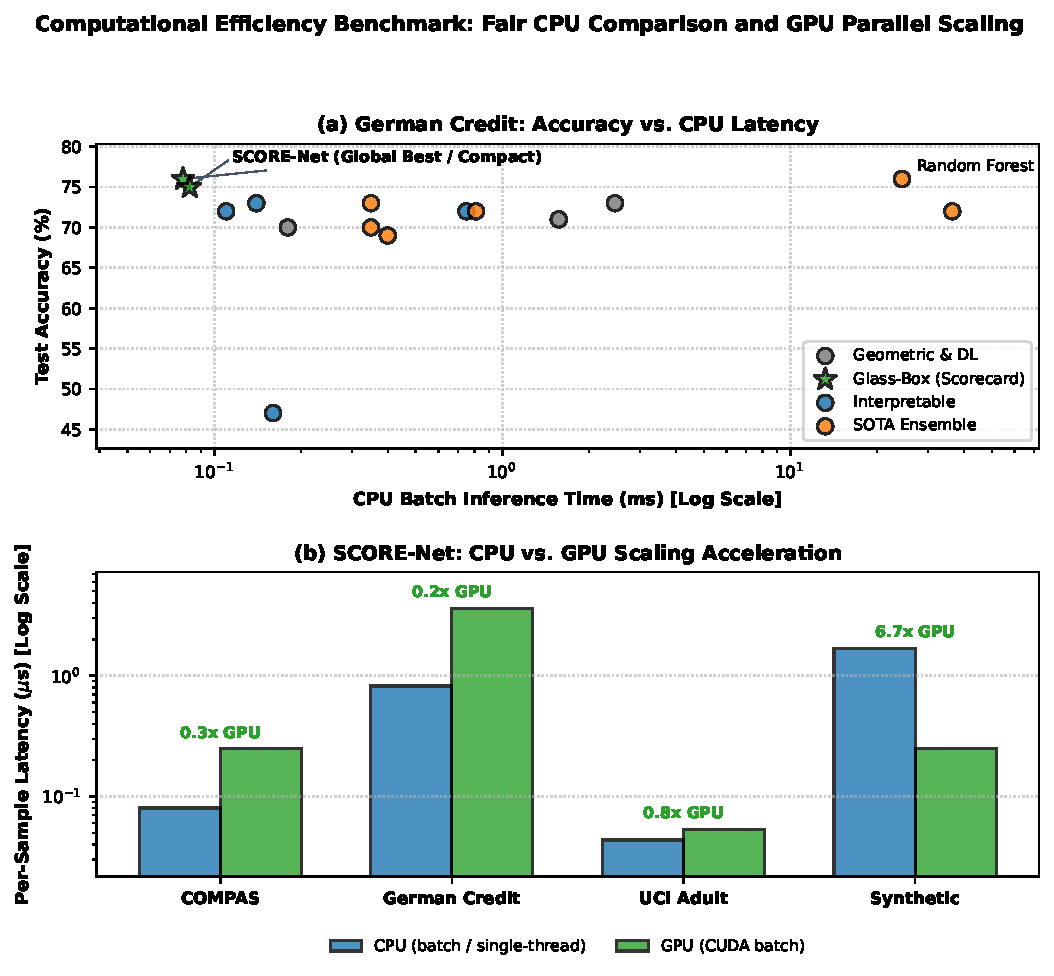
\includegraphics[width=0.72\textwidth]{figures/fig_inference_speed_benchmark.pdf}
\caption{Host-CPU latency versus accuracy on German Credit (top) and CPU versus
GPU per-sample latency of \modelname{} across datasets (bottom). The top panel
plots the amortized batch cost of Table~\ref{tab:cpu_latency_baselines}, so
\modelname{} sits at the low-latency end of the accuracy range; the bottom panel
uses the throughput-equivalent cost, where CPU suits single-sample scoring and
GPU batching pays off only for large batches.}
\label{fig:supp_inference}
\end{figure}

\section{Rule-List Learners}
\label{sec:supp_rulelist}

The 13 main baselines do not include a method that returns an explicit rule list,
which is the closest family conceptually. We therefore ran two established rule
learners from \texttt{imodels} on the same partitions: RuleFit, which extracts
rules from boosted trees and fits a sparse linear model over them, and a
Skope-rules style conjunction miner. RuleFit reaches 66.67\%, 69.00\% and
83.27\% on COMPAS, German Credit and UCI Adult; the conjunction miner reaches
54.95\%, 30.00\% and 75.21\%. The Global Best variant of \modelname{} exceeds the
stronger of the two on every dataset (68.33\%, 76.00\% and 85.30\%). The Compact
variant also leads on German Credit (75.00\%) and UCI Adult (85.61\%), but it is
0.35 points below RuleFit on COMPAS (66.32\% versus 66.67\%), which we report as
measured. Neither learner supports the 20-class task, so no comparison is
possible on Synthetic. These results are reported separately because the
families differ in what they guarantee: RuleFit returns rules but not a bounded
slab per unit, and it provides no exact compaction step.

\section{Scorecard Quantization Detail}
\label{sec:supp_quantization}

Figure~\ref{fig:supp_scorecard} shows the two scaling regimes of
the quantization section of the main text for the German Credit Compact model. A small
uniform multiplier rounds many weights to zero and destroys accuracy, whereas a
large one inflates the integer range; the rule-adaptive search instead selects
the smallest multiplier per rule that meets the rounding tolerance, which keeps
the integer weights inside $[-5,6]$.

\begin{figure}[H]
\centering
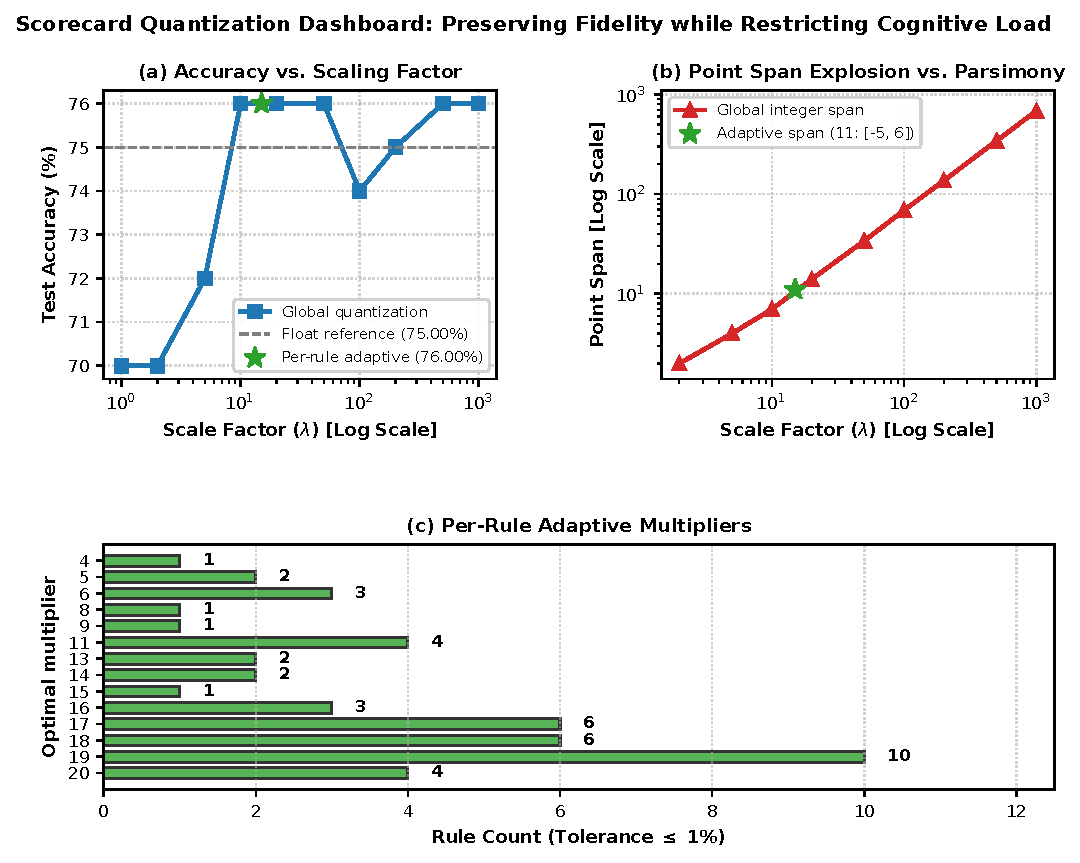
\includegraphics[width=0.68\textwidth]{figures/fig_scorecard_dashboard.pdf}
\caption{Scorecard quantization on German Credit (Compact model). (a) Test
accuracy as a function of a uniform global scaling factor $\lambda$; the dashed
line is the unquantized float model (75.00\%) and the star is the per-rule
adaptive operating point (76.00\%). (b) Integer point span produced by a global
scale grows roughly linearly with $\lambda$, whereas the adaptive rule-level
choice confines the integer weights to $[-5,6]$. (c) Distribution of the selected
per-rule multipliers $\lambda_h^\ast$ over the 46 surviving rules (mean 15.00).}
\label{fig:supp_scorecard}
\end{figure}

\section{Decision Diagnostics on German Credit}
\label{sec:supp_diagnostics}

This section collects the three diagnostic tools that the main text summarizes
in its case-study section: exact response curves, closed-form recourse, and
architectural feature co-occurrence. Each is computed analytically from the same Compact
checkpoint, without sampling or surrogate models.

\subsection{Exact Response Curves}
Figure~\ref{fig:supp_response} evaluates a rejected applicant whose decision
margin is $-0.54$, the median margin among rejected test applicants. For
\textit{duration} the applicant sits at $+0.25$ standard deviations inside the
rejected region, and reducing it below $-0.17$ crosses the boundary, so a shift
of $-0.42$ suffices for approval. For \textit{credit\_amount} the response is
non-monotone: the margin turns positive on roughly $[0.69, 1.87]$ and negative
again beyond, because two rules with opposite votes overlap there.

\begin{figure}[H]
\centering
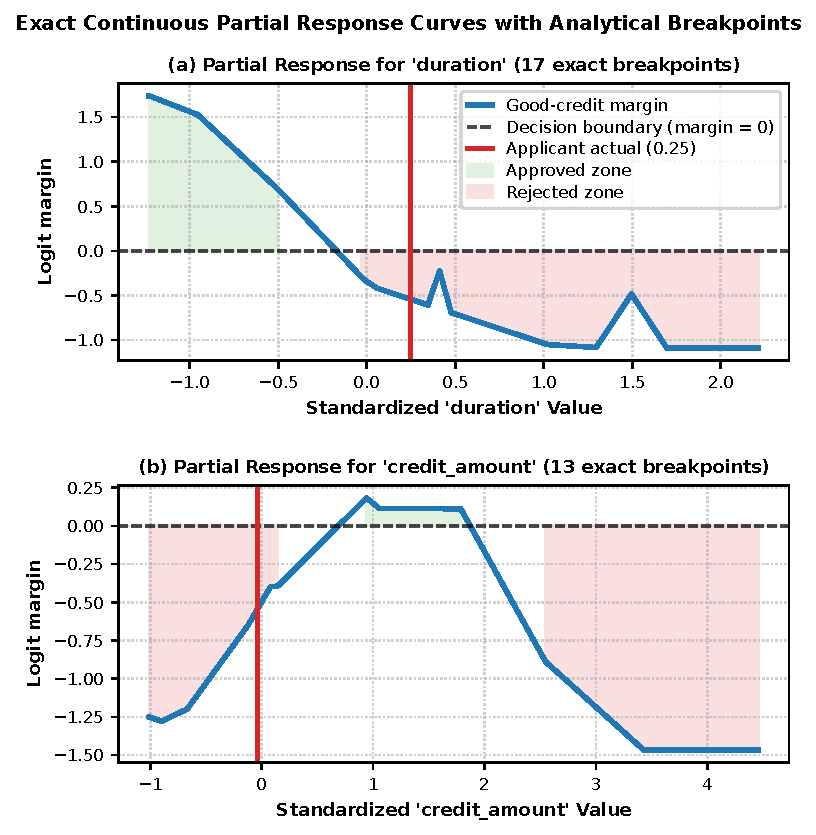
\includegraphics[width=0.55\textwidth]{figures/fig_local_feature_curves.pdf}
\caption{Exact conditional response curves for a rejected German Credit applicant
(decision margin $-0.54$). Each curve is evaluated only at the algebraic
breakpoints of the piecewise-linear model, so it carries no sampling or
interpolation error; the number in each panel title is the resulting count.
(a) \textit{duration}: shortening the loan crosses the boundary at $-0.17$
standard deviations. (b) \textit{credit\_amount}: the response is non-monotone and
contains an approval corridor around $[0.69, 1.87]$.}
\label{fig:supp_response}
\end{figure}

\subsection{Closed-Form Recourse}
Figure~\ref{fig:supp_recourse} lists the independent single-feature
interventions that are each sufficient to flip the same applicant to approval.
Age, marital status/sex and foreign-worker status are held fixed, and only
interventions inside the observed training range are admitted. The smallest
interventions are a reduction of \textit{residence\_since} by 0.35 standard
deviations, a reduction of \textit{duration} by 0.42, an increase of
\textit{property\_magnitude} by 0.45, and a change of \textit{purpose} from
``new car'' by 0.48; the remaining bars require between 0.51 and 0.80 units.
Because each root solves a piecewise-linear equation, the shifts are exact for
the model and reproducible. They remain \emph{geometric} candidates: feasibility
is a domain and causal question that the model cannot answer.

\begin{figure}[H]
\centering
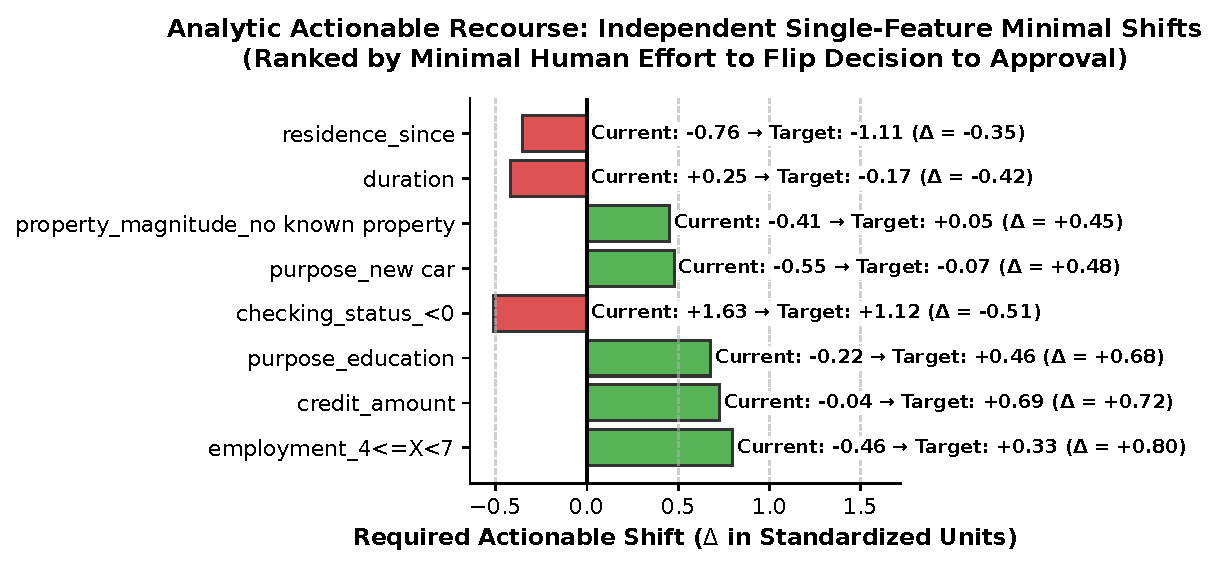
\includegraphics[width=0.7\textwidth]{figures/fig_actionable_recourse.pdf}
\caption{Closed-form single-feature recourse for the applicant of
Figure~\ref{fig:supp_response}. Each bar is an independent intervention that is
sufficient on its own to reverse the decision, ranked by the required change in
standardized units. Immutable attributes (age, marital status/sex, foreign-worker
status) are excluded from the search.}
\label{fig:supp_recourse}
\end{figure}

\subsection{Architectural Feature Co-occurrence}
Figure~\ref{fig:supp_cooccurrence} shows the co-occurrence structure of the ten
most frequently used German Credit features. Off-diagonal Jaccard similarities
are at most 0.33 (\textit{residence\_since} with \textit{purpose\_radio/tv}),
followed by 0.25 (\textit{purpose\_new car} with \textit{credit\_history\_no
credits/all paid}) and 0.22 (\textit{checking\_status\_no checking} with
\textit{savings\_status} $\ge 1000$). The near-diagonal structure is consistent
with the average rule length of 2.70 features: pruning has decoupled most
features into short, individually auditable rules rather than a dense web of
interactions. The measure is structural and model-derived; it is not a causal
interaction test.

\begin{figure}[H]
\centering
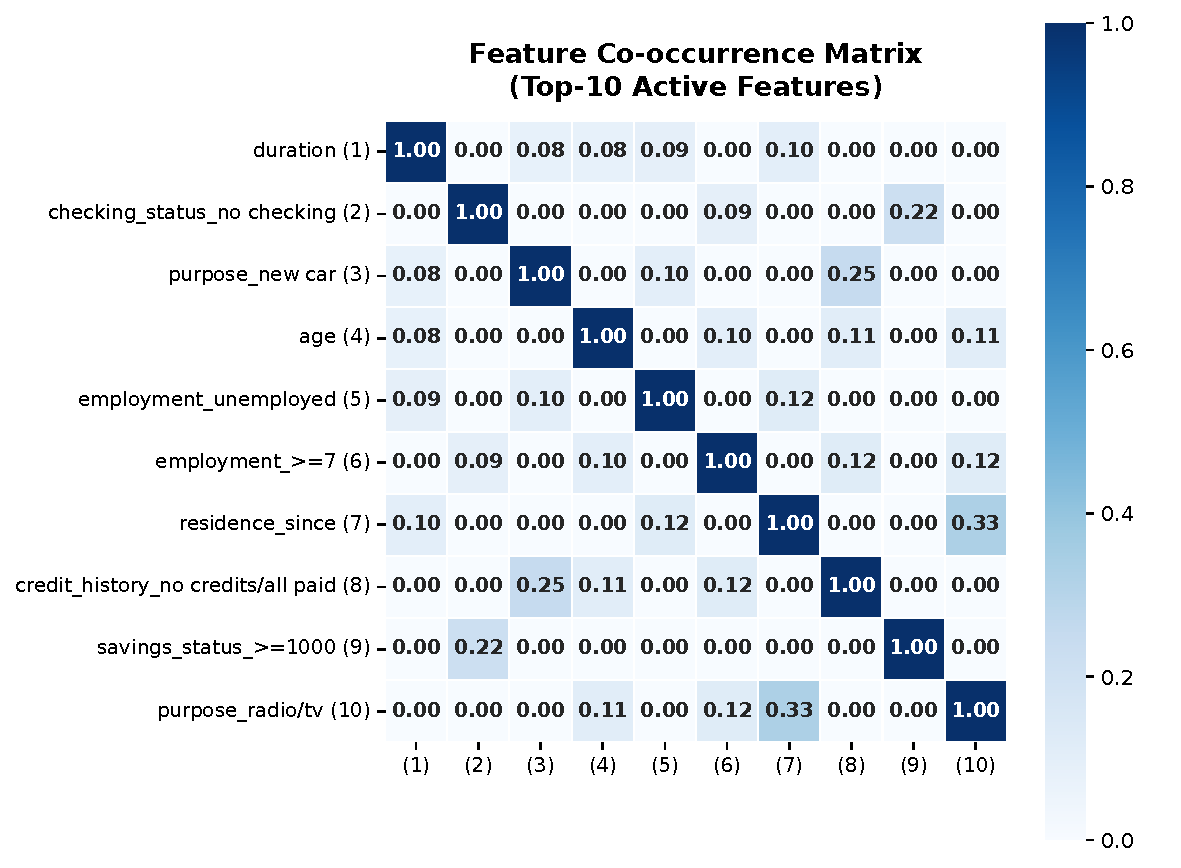
\includegraphics[width=0.7\textwidth]{figures/fig_feature_interaction.pdf}
\caption{Architectural feature co-occurrence and pairwise Jaccard similarity for
the ten most active features of the German Credit Compact model. Off-diagonal
values are at most 0.33, reflecting the short average rule length (2.70
features).}
\label{fig:supp_cooccurrence}
\end{figure}

\section{Ablation Figure}
\label{sec:supp_ablation}

Figure~\ref{fig:supp_ablation} plots the ablation results of the ablation table in the main
text. Panel (a) shows the effect of removing each loss component on test
accuracy and on the number of surviving rules; panel (b) shows how the initial
capacity $H$ trades rule count against accuracy.

\begin{figure}[!htb]
\centering
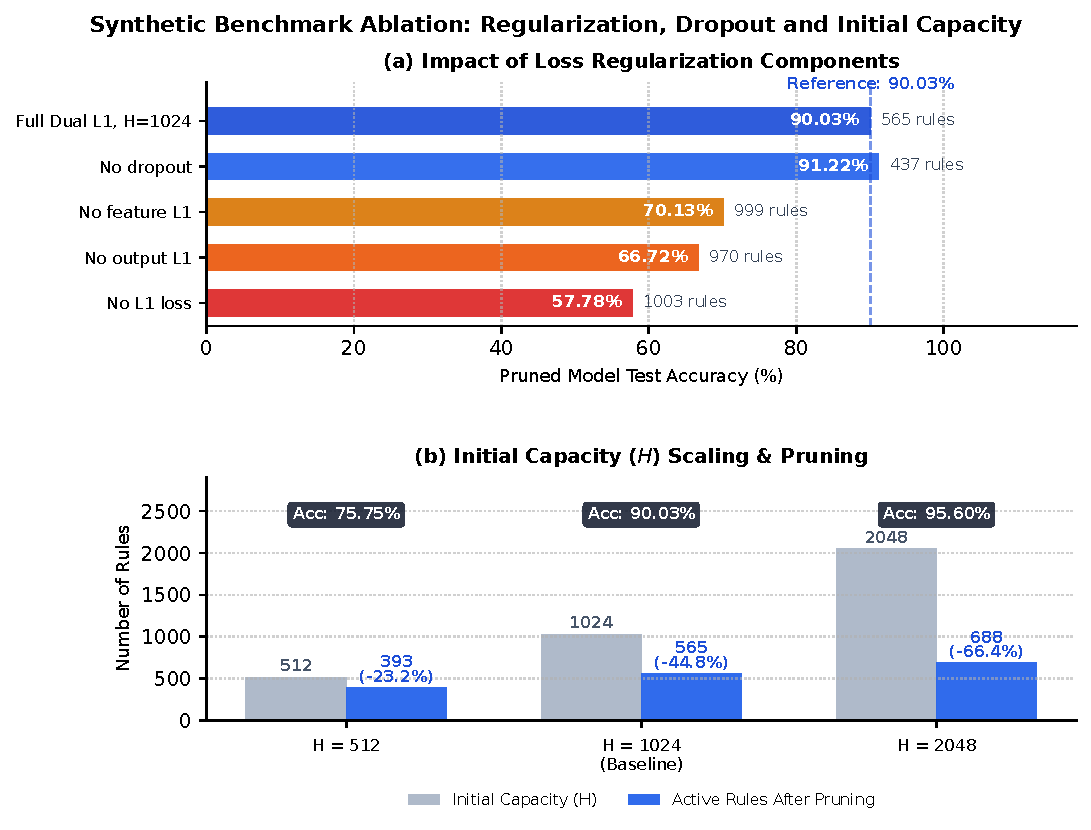
\includegraphics[width=1\textwidth]{figures/fig_ablation_synthetic.pdf}
\caption{Ablation on the 20-class Synthetic benchmark. (a) Test accuracy and
surviving rule count for the full model and for variants with individual loss
components removed. (b) Effect of the initial capacity $H$ on the number of
surviving rules and on test accuracy.}
\label{fig:supp_ablation}
\end{figure}

\end{document}
